\documentclass{article}
\usepackage{paper}

\setpapertitle{Discrete Variational Autoencoders and Stochastic Block Models}

\newcommand{\pp}{p\para}
\newcommand{\qp}{q\para}
\newcommand{\rp}{r\para}

\begin{document}
\makeheader

\abstract{
	Many latent variable models like variational graph autoencoders have been proposed recently for link prediction in graphs, however they provide little or no interpretability of the node representations. In contrast, variants of the Stochastic Block Models (SBMs) such as the mixed-membership model and non-parametric latent feature relational models have been successful in providing interpretable latent features along with adroitly discovering community structure. In an attempt to unify these two strands of research, this work presents an enhanced variational autoencoder model for graphs, with each node modelled as a binary latent vectors with an expressive restricted Boltzmann machine (RBM) prior. To handle the intractable inference, we leverage the Gumbolt reparametrization, along with continuous latent representations to retain the interpretability while still retaining excellent predictive power of these representations. We will also present a brief survey of some of the state of the art models for using binary latent variables in the variational inference literature, followed by some experimental results on the behaviour of these models.
}
\begin{psection}{Introduction}

	With the increasing importance of analyzing social networks, there has been a lot of work on link prediction for graphs or relational data.

	Learning vector-valued node representations (a.k.a.  embeddings) is a fundamental task in many problems involving graph-structured data. In a probabilistic modelling setting, we can learn these by treating the embeddings as latent variables and assuming that the graph adjacency matrix is generated via the interactions of these latent variables. Recent works, such as \cite{gvae} offer excellent predictive properties for this task, however, the caveat with using such models is the continuous nature of the latent representations, as these tend to not be interpretable.

	Some models such as the Stochastic Block Model and its variants afford interpretable embeddings, but either suffer from low predictive power, or slow inference. In this work, these two approaches are combined to present a novel model which retains the predictive expressiveness of continuous latent variables, while simultaneously presenting interpretable latent variables.

\end{psection}

\begin{psection}{Background}

	\begin{psubsection}{Black Box Variational Inference}

		Black Box Variational Inference \citep{bbvi} is based on stochastic optimization of the variational objective. This allows us to perform model free analysis, which standard variational inference does not afford. Black box inference estimates the gradients of the variational objective (the ELBO) using Monte Carlo samples from the proxy posterior distribution. This can be derived by computing the gradients of the ELBO, which is written as below.
		\begin{align}
			\elbo{\vx, \vphi}	&\eq \E[\vz \sim q(\vz \spipe \vx, \vphi)]{\logp{p(\vx, \vz)} - \logp{q(\vz \pipe \vx, \vphi)}} \\
			\implies \nabla \elbo{\vx, \vphi} &\eq \E[\vz \sim q(\vz \spipe \vx, \vphi)]{\nabla_\vphi \logp{q(\vz \pipe \vx, \phi)} \para{\logp{p(\vx, \vz)} - \logp{q(\vz \pipe \vx, \vphi)}}} \label{eq:score-function}
		\end{align}

		The derivation of the above transformation can be found in the original paper by \cite{bbvi}. Since we formulated the gradient of the ELBO as an expectation, we can now use Monte Carlo estimation to get unbiased estimates of the ELBO gradient. This method is popular for the generality of the method, as it can be applied on most posterior estimation problems, with very few restrictions. However, the gradient estimates computed using this method have high variance, and therefore are often unsuitable to use in practical scenarios.

		Many suggestions have been posed to overcome the variance problem. Most of them have common themes, and can be loosely classified as the following three classes
		\begin{enumerate}
			\item \ditem{Control Variates} Control variates are stochastic terms added to the monte carlo estimates so as to reduce the variance, while preventing any extra bias in the estimates. \cite{cv-johnson}, \cite{cv-paisley}, \cite{cv-chong} and \cite{bbvi} present some techniques to reduce variance in BBVI gradient estimates using control variates.

			\item \ditem{Non-uniform Sampling} The idea behind non-uniform sampling is based on selecting mini-batches which produce low variance estimates of the ELBO gradient. These samples are assigned higher probability of sampling, and therefore non-uniform sampling is employed. Works by \cite{nus-dominik}, \cite{nus-prem}, \cite{nus-volkan}, etc. fall under this category.

			\item \ditem{Reparametrization} The reparametrization trick allows estimation of the ELBO gradients using samples from a noise distribution with an apt (deterministic) transformation from the noise variable to the latent variable in question. Reparametrization trick reduces the variance by much, and is most desirable in many cases.

				This trick was successfully used by \cite{vae} for amortized inference, by transorming the gaussian latent variables as a deterministic mapping from the random normal noise variable to the desired distribution. The reparametrization trick is of much interest, and I probe deeper into the many methods for reparametrization in Black Box Variation Inference, before moving towards studying black box inference of discrete latent variable models (with reparametrization).

				Another problem with reparametrization is that it disallows the use of discrete latent variables. This is discussed in more detail in later sections.
		\end{enumerate}

		Another popular technique to reduce variance relies on Rao Blackwellization, also used by \cite{bbvi} to reduce variance for the standard BBVI gradient estimates.

	\end{psubsection}

	\begin{psubsection}{Reparametrization for BBVI}

		The formulation written in equation \ref{eq:score-function} is known as the Score Function method. In order to reparameterize, the latent variable is written as a deterministic transformation of a noise variable (say $\vepsilon$) using a function $f$ such that $\vz = f(\vepsilon)$. Equation \ref{eq:score-function} can then be written alternately as
		\begin{align}
			<++>\nabla \elbo{\vx, \vphi} \eq \E[\vepsilon]{\nabla_{\vphi} \logp{q(f(\vepsilon) \pipe \vx, \vphi)} \para{\logp{p(\vx, f(\vepsilon)) - \logp{q(f(\vepsilon) \pipe \vx, \vphi)}}}}<++>
			\label{eq:rep-trick}
		\end{align}

		The biggest problem with the reparametrization trick is the limited number of distributions to which the trick can be applied successfully. Moreover, this often includes model specific changes and therefore undermines the Block Box property of BBVI. There have been attempts to remedy this by allowing general reparametrization methods.

		\cite{gen-rep-grad} presents a generic reparameterization method for a large class of distributions by mapping the latent variables to random variables which are assumed to be only weakly dependent on the parameters of the posterior. Although this allows us to reparametrize a much greated class of models, however, this still requires finding random variables and commensurate invertible mapping for weak dependence.

		\cite{implicit-rep-grad} further builds upon generalized reparameterization \citep{gen-rep-grad} by introducing implicit differentiation \ie differentiation without explicitly inverting the mapping function between the latent and reparameterization variables. This allows for better convergence properties.

		Another generic reparametrization technique is reparameterization through acceptance/rejection sampling \citep{rep-acc-rej}. Since reparameterization only allows deterministic mapping from reparameterization variables to the latent variables, this technique augments reparameterization for variables sampled using Accept/Reject algorithms.

		The common problem among all these methods is the incapability to handle discrete latent variables. In fact, it is not possible to use reparametrization with discrete latent variables. Therefore, score function methods need to be used, however, they have such a high variance they are practically unusable.

	\end{psubsection}

	\begin{psubsection}{Discrete Latent Variables and BBVI}

		Although it is theoretically possible to learn models with discrete latent variables using the Score Function method, however, this naive approach gives estimates of the gradients which are impractically high variance. This variance can be reduced by adding control variates, which essentially translates to the \st{Reinforce} strategy (a technique popular in the Reinforcement Learning framework).

		Even with this reduced variance, we still face other difficulties. As \cite{dvae} points out, to capture an efficient estimate of the variance of a D-dimensional latent variable, we need at least D samples. Since a model can effectively have 100s of latent variables, the number of samples required to estimate the gradients is huge, and therefore inefficient. On the contrary, when using reparametrization, even a single sample can effectively estimate the direction of the gradients, and therefore work effeciently in training such models.

		Most methods to train models with discrete latent variables follow under one of five classes.
		\begin{enumerate}
			\item <++> Exhaustive approaches marginalize all discrete variables [25, 26] and which are not scalable to more than a few discrete variables.
			\item Local expectation gradients [27] and reparameterization and marginalization [28] estimators compute low-variance estimates at the cost of multiple function evaluations per gradient. These approaches can be applied to problems with a moderate number of latent variables.
			\item Relaxed computation of discrete densities [29] replaces discrete variables with continuous relaxations for gradient computation. A variation of this approach, known as the straight-through technique, sets the gradient of binary variables to the gradient of their mean [30, 31].
			\item Continuous relaxations of discrete distributions [32] replace discrete distributions with con- tinuous ones and optimize a consistent objective. This method cannot be applied directly to Boltzmann distributions. The DVAE [19] solves this problem by pairing each binary variable with an auxiliary continuous variable. This approach is described in Sec. 2.
			\item The REINFORCE estimator [33] (also known as the likelihood ratio [34] or score-function estimator) replaces the gradient of an expectation with the expectation of the gradient of the score function. This estimator has high variance, but many increasingly sophisticated methods provide lower variance estimators. NVIL [3] uses an input-dependent baseline, and MuProp [35] uses a first-order Taylor approximation along with an input-dependent baseline to reduce noise.  VIMCO [36] trains an IWAE with binary latent variables and uses a leave-one-out scheme to define the baseline for each sample. REBAR [37] and its generalization RELAX [38] use the reparameterization of continuous distributions to define baselines.
			<++>
		\end{enumerate}

		In the following sections, I discuss some methods to translate discrete latent variables to continuous variables, using smoothing techniques. For each relaxation, there lies a concomitant reparametrization method for fast inference and low variance estimates for the ELBO gradient. This discussion is mostly centered around binary latent variables.

	\end{psubsection}

	\begin{psubsection}{Restricted Boltzmann Machines}

		A boltzmann machine is an undirected probabilistic energy based model, where the probability mass for a binary (vector) latent variable, $\vz$, is given by
		\begin{align}
			\prob{\vz} \eq \frac{\texp{- E_\vtheta(\vz)}}{Z_\vtheta}
			\label{eq:bm-prob}
		\end{align}
		where $E_\vtheta(\vz)$ is the energy function, and $Z_\vtheta$ is the partition function, given by
		\begin{align*}
			Z_\vtheta \eq \sum_{\set{\vz}} \texp{- E_\vtheta(\vz)}
		\end{align*}

		Since the dimension of the variable $\vz$ can be large, it is impractical to compute the partition function, and therefore sampling needs to be used to estimate the value. In order to allow easier sampling (using Blocked Gibbs Sampling), we often assume the relation (undirected) between variables to be bipartite. This means that the set of variables $\vz$ is divided into two parts, $(\vz_1, \vz_2)$, and it is assumed that there is no link among the variables in $\vz_1$ and $\vz_2$ separately. This effectively means that given $\vz_1$, the probability of each variables in $\vz_2$ is independent, and vice versa. Such a model is known as the Restricted Boltzmann Machine (RBM). In the RBM literature, the variables $\vz$ are divided into visible and hidden variables, however since the models I discuss use RBMs as priors, we omit such distinction between the two sets of latent variables.

		The energy function in case of RBMs is given as
		\begin{align}
			E_\vtheta(\vz) \eq \va \cdot \vz_1 + \vb \cdot \vz_2 + \trans{\vz_2} \sW \vz_1
			\label{eq:energy-function}
		\end{align}
		where $\va$, $\vb$ and W are the biases (on $\vz_1$ and $\vz_2$ , respectively) and weights.

	\end{psubsection}

\end{psection}

\begin{psection}{Gumbel-Softmax Trick}

	The Gumbel-Softmax Trick \citep{concrete, gumbel} affords a smooth relaxation for categorical variables, based on the Gumbel distribution and the Sofmax trick (and hence the name).

	Typically, sampling from a bernoulli involves firstly sampling from a uniform random variable (from 0 to 1), U and return the categorical variable C (with say, $K$ classes) as follows
	\begin{align*}
		\sC \eq \argmin{k \in \brac{K}} \sU - \sum_{k' = 1}^k \pi_{k'}
	\end{align*}

	\note{The parameters $\set{\pi_k}_{k = 1}^K$ denote the probabilities of each class for the categorical distribution, and therefore $\sum_{k = 1}^K \pi_k = 1$. Below, I alternately use weights $\set{\alpha_k}_{k = 1}^K$ instead of probabilities, and therefore, we will have $\pi_k = \frac{\alpha_k}{\sum_{k' = 1}^{K} \alpha_{k'}}$}

	An alternate way, however, to sample from the categorical distribution is by using the Gumbel-Max trick (upon which the Gumbel-Softmax is based). The Gumbel-Max trick says that in order to sample from a categorical distribution with weights $\set{\alpha_k}_{k = 1}^K$, we sample $K$ uniform random variables $\set{\sU_k}_{k = 1}^{K}$ and reparametrize as follows
	\begin{align*}
		\sC \eq \argmax{k \in \brac{K}} \logp{\alpha_k} - \log{- \log{\sU_k}}
	\end{align*}

	The variable $-\log{-\log{U}}$ is known to be from the Gumbel disitribution. This alternate sampling strategy allows us to write the relaxed version of the random variable C (denoted by $\vZ = \brac{\sZ_1 \dots \sZ_K}$). which is then given as
	\begin{align*}
		\sZ_k \eq \frac{\texp{\para{\logp{\alpha_k} + \sG_k} / \tau}}{\sum_{k' = 1}^K \texp{\para{\logp{\alpha_{k'}} + \sG_{k'}} / \tau}}
	\end{align*}
	where $\sG_k$ is a sample from the gumbel distribution, and $\tau$ is a parameter, known as the temperature. It is obvious to see that as $\tau \ra 0$, the smooth relaxation $Z_k \ra \is{C = k}$.

	In the ELBO term, the terms for the prior and posterior of the latent variable C are replaced by simple relaxations to facilitate proper inference of the objective. This can be easily used to train binary latent variables, which is also shown in detail in \cite{concrete}. The problem, however, is that this relaxation is limited to simple categorical priors, and therefore does not scale to more complicated priors such as the Boltzman Machine prior.

	In the following sections, some of the popular methods to infer models with Boltzman priors are discussed. These methods use alternate relaxations, which allow us to use better priors.

\end{psection}

\begin{psection}{Discrete Variational Autoencoders}

	\cite{dvae} proposed models with RBM priors within the variational autoencoder framework. Although \cite{dvae} propose a model with autoregressive connections between the latent variables $\vz$, thereby forming a hieararchy (in the posterior), we assume this to absent in our model. This simplifies the discussion and allows us to focus on the discussion pertaining to inference with binary latent variables.

	In order to allow inference, the model is augmented with continuous variables $\vzeta$ as shown in Figure \ref{fig:dvae-network}. Note, the model assumes that in the generative network, the observed labels $\vx$ only depend on the smooth analogs of the latent variables, \ie $\vx$ only depend on $\vzeta$.

	\begin{figure}[htpb]
		\begin{subfigure}[b]{0.5\textwidth}
			\centering
			\begin{tikzpicture}[->, >=stealth', shorten >=1pt, auto, node distance=1.8cm, semithick]
				\node[state]	(x)				 	{$\vx$};
				\node[state]	(z2) [below of=x]	{$\vz_2$};
				\node[state]	(z1) [left of=z2]	{$\vz_1$};
				\node[state]	(z3) [right of=z2]	{$\vz_3$};
				\node[state]	(c1) [below of=z1]	{$\vzeta_1$};
				\node[state]	(c2) [below of=z2]	{$\vzeta_2$};
				\node[state]	(c3) [below of=z3]	{$\vzeta_3$};

				\path	(x)		edge	node	{}	(z1)
								edge	node	{}	(z2)
								edge	node	{}	(z3)
						(z1)	edge	node	{}	(c1)
						(z2)	edge	node	{}	(c2)
						(z3)	edge	node	{}	(c3);
			\end{tikzpicture}
			\caption{Posterior Network ($\qp{\vzeta, \vz \pipe \vx}$)}
			\label{fig:dvae-network:posterior}
		\end{subfigure}
		\begin{subfigure}[b]{0.5\textwidth}
			\centering
			\begin{tikzpicture}[->, >=stealth', shorten >=1pt, auto, node distance=1.8cm, semithick]
				\node[state]	(z2)			 	{$\vz_2$};
				\node[state]	(z3) [right of=z2]	{$\vz_3$};
				\node[state]	(z1) [left of=z2]	{$\vz_1$};
				\node[state]	(c1) [below of=z1]	{$\vzeta_1$};
				\node[state]	(c2) [below of=z2]	{$\vzeta_2$};
				\node[state]	(c3) [below of=z3]	{$\vzeta_3$};
				\node[state]	(x)  [below of=c2]	{$\vx$};

				\draw[-] ;

				\path	(z1)	edge						node	{}	(c1)
								edge [-]					node	{}	(z2)
								edge [-, out=30, in=150]	node	{}	(z3)
						(z2)	edge						node	{}	(c2)
								edge [-]					node	{}	(z3)
						(z3)	edge						node	{}	(c3)
						(c1)	edge						node	{}	(x)
						(c2)	edge						node	{}	(x)
						(c3)	edge						node	{}	(x);
			\end{tikzpicture}
			\caption{Prior Network ($\pp{\vzeta, \vz}$)}
			\label{fig:dvae-network:prior}
		\end{subfigure}
		\caption{Graphical Models of the approximating posterior (a) and the prior (b)}
		\label{fig:dvae-network}
	\end{figure}

	We can write the same mathematically, with the prior $p(\vzeta, \vz \pipe \vtheta)$ as follows
	\begin{align}
		\pp{\vzeta, \vz \pipe \vtheta}	&\eq r\para{\vzeta \pipe \vz} \cdot \pp{\vz \pipe \vtheta}, \hspace{1cm}\mt{where}
		\label{eq:dvae-prior} \\
		r\para{\vzeta \pipe \vz}			&\eq \prod_i r\para{\zeta_i \pipe z_i} \nonumber
	\end{align}
	The posterior is correspondingly augmented as follows
	\begin{align}
		\qp{\vzeta, \vz \pipe \vx, \vphi}	&\eq	r\para{\vzeta \pipe \vz} \cdot \qp{\vz \pipe \vx, \vphi}
		\label{eq:dvae-post}
	\end{align}
	The distribution $r(\vzeta \pipe \vz)$ is the same for both the posterior and the prior. Although the following discussion is generic and can be applied to any probabilistic model, we restrict the notation to that for variational autoencoders. Similar to Variational Autoencoders, we can write the ELBO as a sum of a KL term and an autoencoding term.
	\begin{align}
		\elbo{\vz, \vphi} \eq \underbrace{- \kld{\qp{\vzeta, \vz \pipe \vx, \vphi}}{\pp{\vzeta, \vz \pipe \vtheta}}}_\text{KL Term} + \underbrace{\E[q(\vzeta, \vz \spipe \vx, \vphi)]{p(\vx \pipe \vzeta, \vtheta)}}_\text{Autoencoding Term}
		\label{eq:elbo-division}
	\end{align}

	The gradient of the autoencoding term can be computed by sampling the latent variables $\vzeta$. This is possible due to reparametrization of the latent variable $\vzeta$, which is discussed later in this section. For the KL term, \cite{dvae} give a very detailed explanation on computing the gradients. However, since I assume the autoregressive connections to be absent from the network, the computation of the KL term greatly simplifies. The gradients for the KL term can be written as
	\begin{align}
		\nabla \kld{q}{p} &\eq \underbrace{\E[q(\vz \spipe \vx, \vphi)]{\nabla E_\vtheta(\vz)} - \E[p(\vz \spipe \vtheta)]{\nabla E_\vtheta(\vz)}}_\text{Gradients for Prior Parameters} + \\
		&\hspace{2cm} \underbrace{\sum_{i} \sum_{z_i} \qp{z_i \pipe \vx, \vphi} \logp{\qp{z_i \pipe \vx, \vphi}} + \nabla E_\vtheta\para{\E[q(\vz \spipe \vx, \vphi)]{\vz}}}_\text{Gradients for Posterior Parameters}
		\label{eq:dvae-kl-grad}
	\end{align}

	\note{The above equation can only be written if the posterior of latent variables $\vz$ is assumed to be such that we can write $\qp{\vz \pipe \vx, \vphi} = \prod_i \pp{z_i \pipe \vx, \vphi}$}

	The gradients for the KL term are independent of the continuous relaxations $\vzeta$, and therefore the only dependency of the gradients is in the autoencoding term, where we need to sample the latent variables $\vzeta$. \cite{dvae} propose a few relaxations, such as the spike-and-exponential relaxation, the spike-and-slab relaxation and the spike-and-gaussian relaxation. I only discuss the spike-and-exp relaxation as it was observed to perform the best.

	\begin{psubsection}{Spike and Exponential Smoothing Transformation}

		The probability density function $\rp{\zeta_i \pipe z_i}$ for spike-and-exp transformation is given as
		\begin{align}
			\rp{\zeta_i \pipe z_i = 0}	&\eq \begin{cases}
				\infty,	& \mt{if} \zeta_i = 0 \\
				0,		& \mt{otherwise}
			\end{cases} \nonumber \\
			\rp{\zeta_i \pipe z_i = 1}	&\eq \begin{cases}
				\frac{\beta \exp{\beta \zeta}}{\exp{\beta} - 1},	& \mt{if} \zeta_i \in \brac{0, 1} \\
				0,													& \mt{otherwise}
			\end{cases}
			\label{eq:spike-and-exp:pdf}
		\end{align}
		The inverse CDF for the same is given (details in the original paper) as
		\begin{align}
			\zeta_i \eq F_{\qp{\zeta_i \spipe \vx, \vphi}}^{-1}(\rho_i)	\eq \max\set{\frac{1}{\beta} \cdot \logp{\brac{\para{\frac{\rho_i + q_i - 1}{q_i}} \cdot \para{\exp{\beta} - 1}} + 1}, 0}
			\label{eq:spike-and-exp:icdf}
		\end{align}
		where $\rho \in \para{0, 1}$ is sampled from a uniform distribution (from 0 to 1), and $q_i$ is the short-hand notation for $\qp{z_i \pipe \vx, \vphi}$.

	\end{psubsection}

	The spike-and-exponential smoothing allows us to effectively use binary latent variables with RBM priors. This approach was extended by \cite{dvae-pp}, where in the spike-and-exp relaxation is replaced by overlapping transformation of two exponential distributions. The main advantage of using this is that exp-and-exp relaxations allow us to use Automatic Differentiation (AD) for learning the model, as opposed to the case in DVAE, where in the gradients (for the KL) need to be manually coded. The reason, as noted by the authors, is the symmetric distribution for $z_i = 0$ and $z_i = 1$. However, this is not observed with the assumption that the posterior decouples over the dimensions of the latent variables $\vz$, as noted above.

	\begin{psubsection}{Overlapping Transformations - Exponential and Exponential Smoothing}

		The probability density function $\rp{\zeta_i \pipe z_i}$ for exp-and-exp transformation, similar to the spike-and-exp case, is given as
		\begin{align}
			\rp{\zeta_i \pipe z_i = 0}	&\eq \begin{cases}
				\frac{\beta \exp{\beta (1 - \zeta)}}{\exp{\beta} - 1},	& \mt{if} \zeta_i \in \brac{0, 1} \\
				0,		& \mt{otherwise}
			\end{cases} \nonumber \\
			\rp{\zeta_i \pipe z_i = 1}	&\eq \begin{cases}
				\frac{\beta \exp{\beta \zeta}}{\exp{\beta} - 1},	& \mt{if} \zeta_i \in \brac{0, 1} \\
				0,													& \mt{otherwise}
			\end{cases}
			\label{eq:spike-and-exp:pdf}
		\end{align}
		The inverse CDF in this case is given (details in the original paper) as
		\begin{align}
			\zeta_i \eq F_{\qp{\zeta_i \spipe \vx, \vphi}}^{-1}(\rho_i)	\eq - \frac{1}{\beta} \cdot \logp{\frac{-b + \sqrt{b^2 - 4ac}}2}
			\label{eq:spike-and-exp:icdf}
		\end{align}
		where $\rho \in \para{0, 1}$ is sampled from a uniform distribution (from 0 to 1), and $b = \brac{\rho + \exp{-\beta}(q_i - \rho)} / (1 - q_i) - 1$, $c = \para{q_i \exp{- \beta}}/(1 - q_i)$, and $q_i$ is the short-hand notation for $\qp{z_i \pipe \vx, \vphi}$.

	\end{psubsection}

	Both \cite{dvae} and \cite{dvae-pp} propose models having binary latent variables with an RBM prior, using smoothing transformations based on spipe-and-exp and exp-and-exp (respectively) transformations. This work was further extended by \cite{dvae-sharp}, wherein a generic strategy was proposed to compute inverse CDF in case of overlapping distributions. They show their methods to work better than DVAE and DVAE++, and propose another overlapping distribution based on power distribution. Although I do not discuss much on their findings, it is an interesting work, exploring which I leave as a future task.

\end{psection}

\begin{psection}{GumBolt Trick}

	As pointed out earlier, the Gumbel Softmax trick is built for factorial distributions and does not scale to RBM priors. \cite{gumbolt} point out that the reason behind this is the removal of the latent variables $\vz$ from the inference model. Therefore, an alternate model, named as GumBolt is suggested by \cite{gumbolt} using the Gumbel-Softmax trick along with RBM priors.

	Similar to gumbel softmax case, a relaxed probabilities are required to replace the prior and the posterior probabilities. The posterior probability is consistent with the reparameterization offered by the Gumbel-Softmax Trick, however, the prior probability is replaced with a proxy, which is given as
	\begin{align}
		\widetilde{p}\para{\vzeta \pipe \vtheta} \eq \frac{\exp{-E_\vtheta(\vzeta)}}{Z_\vtheta}
		\label{eq:gumbolt-prob-proxy}
	\end{align}
	where $Z_\vtheta$ is the partition function for the prior probability of $\vz$. Note, the above proxy is not really a probability distribution, as it is unnormalized, however, as the temperature (of the Gumbel-Softmax trick) limits to 0, the above proxy tends to $\pp{\vz \pipe \vtheta}$. Moreover, the inconsistency of the posterior remaining a probability density function even when the temperature parameter limits to 0 is solved by replacing the posterior with a relaxed probability given as $\logp{\widetilde{q}\para{\vzeta \pipe \vx, \vphi}} = \vzeta \cdot \log{q} + (1 - \vzeta) \cdot \log{1 - q}$, where $q$ is the short-hand notation for $\qp{\vzeta \pipe \vx, \vphi}$. Therefore, the relaxed ELBO is written as
	\begin{align}
		\widetilde{\cL}(\vx, \vphi) \eq \E[\qp{\vzeta \spipe \vx, \vphi}]{\logp{\frac{\exp{-E_\vtheta(\vzeta)} \pp{\vx \pipe \vzeta, \vtheta}}{\widetilde{q}\para{\vzeta \pipe \vx, \vphi}}}} - \logp{Z_\vtheta}
		\label{eq:gumbolt-elbo}
	\end{align}

	As the temperature, $\tau \ra 0$, the $\widetilde{\cL}(\vx, \vphi) \ra \elbo{\vx, \vphi}$. The authors prove this ELBO to be a lower bound on the actual ELBO, and therefore claim that optimizing this ELBO with annealing temperature optimizes the actual object. This approach has another advantage over the Gumbel Softmax trick, this being that the Gumbolt proxy ELBO allows the use of importance weighted samples \citep{iwae}, which has shown to converge better than the standard ELBO, as it is an upper bound on the traditional ELBO. Use of RBM priors and Importance Weighted samples gives Gumbolt models an upperhand over the standard VAE with the Gumbel-Softmax Trick. Moreover, the authors empirically show that Gumbolt performs better than DVAE and DVAE++, therefore proving itself to be a fecilitous approach to learning models with binary latent variable.s

\end{psection}

\begin{psection}{Stochastic Block Models}

	A Stochastic Block Model is a generative model for graphs, where the modes are categorized into communities. Essentially, one can interpret the community of a node as the latent feature / latent representation, and the the connections between the nodes as the observed variables. The most basic Stochastic Block model partitions the set of vertices into K communities, and defines the probability of a link between the nodes of these communities. This can be inferred using an EM style framework, with the global variables being the links between nodes and the local/latent variables being the community structure.

	The essential problem between this model and other models derived from the SBM is the limitation of the feature representations. The number of classes to capture the communities and the subcommunities can be very large. Moreover, these models assume a simplistic probability function, with a fixed probability for a link between two communities. The first problem can be resolved using binary vectors as latent variables.

	The second problem, however, is resolved by assuming more expressive latent variables. One such solution is presented by \cite{gvae}, where in a Graph Convolution Network is used as an encoder in the variational autoencoder framework, and the reconstructed links are used for predictions. This model, however, has its own problems pertinent to the non-interpretability of the continous latent variables (normal, as in a standard VAE).

	Both these problems were simultaneously tackled by \cite{sbm-gnn}, an unpublished work, where in binary latent variables are used in company with gaussian variables to interpretability, while maintaining the expressiveness of continous latent variables. This work is an extension of the Non-parametric Latent Feature Relational Model \citep{nlfrm} which uses an Indian Buffet Process (IBP) prior over the latent variables, however uses the same architecture as the standard SNM, and is therefore more difficult to train. \cite{sbm-gnn} uses the same IBP prior for the latent variables, however, the latent variables are assumed to be independent, and therefore sub-community structures cannot be efficiently generated using these priors. I propose to solve this by using an RBM prior over the binary variables, forgoing the non-parametric nature, but adding additional expressiveness to the latent variables. I name this model as Gumbolt Variational Graph Convolutional Network (Gumbolt-VGCN), attributing the name to the use of the Gumbolt Trick along with Graph Variational Autoencoders.

\end{psection}

\begin{psection}{Gumbolt Variational Graph Autoencoder}

	As mentioned in the previous section, for each node, we have a latent representation based on a combination of two types of variables, a binary vector and a real vector. Using the same notation as \cite{sbm-gnn}, we denote the binary latent variable for the n\tth node as $\vb_n$, where $\vb_n \in \set{0, 1}^K$ and the gaussian latent variable as $\vr_n$ and $\vr \in \bR^K$. The latent representation for the n\tth node, then, is given as $\vz_n = \vb_n \odot \vr_n$. Using the VAE architecture, we model the posterior of latent variables through an encoder network based on graph convolutional networks. We first describe the structure of the decoder in the following section.

	\note{Unlike \cite{sbm-gnn} and \cite{nlfrm}, $K$, \ie the number of latent dimensions is fixed, and not learnt using a non-parameteric prior}

	\begin{psubsection}{The VAE Decoder}

		The prior for the binary latent variables is given using an RBM machine. The variables are, therefore, decomposed into two sets, hidden and visible as $\vb = \brac{\vb_1, \vb_2}$, and are then sampled from an RBM prior as follows
		\begin{align}
			\vb_1, \vb_2 \qsim \text{RBM}(\va_1, \va_2, \sW)
			\label{eq:gvgcn-prior-binary}
		\end{align}
		The continuous variables, as mentioned before, are assumed to be sampled from a standard gaussian distribution as follows
		\begin{align}
			\vr \qsim \ND{\vzero, \vI}
			\label{eq:gvgcn-prior-binary}
		\end{align}

		The connections between nodes are then modeled as bernoulli random variables, assumed to be independent when conditioned on the latent variables. More formally, given the latent features $\vz$, we can sample the links between two nodes $n$ and $m$ as
		\begin{align}
			\sA_{nm} \eq \text{Bernoulli}\para{\sigma\para{\trans{\vf_n} \vf_m + c}}
			\label{eq:gvgcn-link}
		\end{align}
		where $\vf_n$ denotes a non-linear transform of the latent representaion $\vz_n$, \ie $\vf_n = \vf(\vz_n)$, and $\vf : \bR^K \ra \bR^{K'}$ is modeled using a neural-network.

	\end{psubsection}

	\begin{psubsection}{The VAE Encoder}

		The encoder is modeled similar to that for a Graph Variational Autoencoder, using a fast, non-iterative recognition model. The parameters used to sample the latent variables $\vb$ and $\vr$ are encoded using a graph convolutional network (GCN). In order to simplify inference, we use the mean field assumption, which assumes conditional independence of the binary and the real latent variables. Essentially, given the feature vector for a node $\vx_n$ and the Adjacecy matrix for the graph $\sA$, we can write the posterior using the mean-field assumption as
		\begin{align}
			\qp{\vb_n, \vr_n \pipe \vx, \sA, \vphi} \eq \prod_{k = 1}^K \qp{b_{n,k} \pipe \vx_n, \sA, \vphi} \qp{r_{n,k} \pipe \vx_n, \sA, \vphi}
			\label{eq:gvgcn-posterior-mean-field}
		\end{align}

		For consistency with the prior, we model the probabilities $\qp{b_{n, k} \pipe \vx, \sA}$ and $\qp{r_{n, k} \pipe \vx, \sA}$ using the bernoulli and the gaussian (respectively) distributions. The parameters for these distributions are generated, as noted above, using a GCN. We write this as
		\begin{align*}
			\qp{b_{n, k} \pipe \vx, \sA, \vphi} &\eq \text{Bernoulli}\para{\pi_{n, k}} \\
			\qp{r_{n, k} \pipe \vx, \sA, \vphi} &\eq \ND{\mu_{n, k}, \sigma_{n, k}^2}
		\end{align*}
		where $\set{\pi_{n, k}, \mu_{n, k}, \sigma_{n, k}}_{k = 1}^K= \text{GCN}(\vx_n, \sA)$.

		In order to infer the parameters, stochastic gradient variational bayes (SGVB) is used. Since this does not support binary (rather, discrete) latent variables, we use the Gumblt Probabilty proxy to compute the gradients ofthe KL term. The samples from the prior are generated using Persistive Contrastive Divergence. This allows us to efficiently train the model, while affording the greater expressive power of RBM priors in a generative setting.

	\end{psubsection}

\end{psection}

\begin{psection}{Experiments}
	Due to the shortage of time, I was only able to conduct limited experiments, with visually analyzing the reconstruction and sampling of MNIST images using Gumbolt-VAE, and performing some experiments with Gumbolt-VGAE.

	The reconstructed and sampled images using Gumbolt-VAE are shown in figure \ref{fig:recon} and \ref{fig:sample}.

	\begin{table}
		\centering
		\begin{tabular}{l c c c c c c}
			\hline
			\multirow{2}{*}{\bt{Method}} & \quad & \multicolumn{2}{c}{\bt{Cora}} & \quad & \multicolumn{2}{c}{\bt{Citeseer}} \\
			& \quad & ROC & AP & \quad & ROC & AP \\
			\hline
			SC				& \quad & 0.8460 & 0.8850 & \quad & 0.8050 & 0.8500 \\
			DW				& \quad & 0.8310 & 0.8500 & \quad & 0.8050 & 0.8360 \\
			LFRM			& \quad & 0.9096 & 0.9060 & \quad & 0.8965 & 0.9118 \\
			VGAE			& \quad & 0.9260 & 0.9328 & \quad & 0.9200 & 0.9200 \\
			\hline
			Gumbolt-VGAE	& \quad & \bt{0.9282} & \bt{0.9396} & \quad & \bt{0.9230} & \bt{0.9339} \\
			\hline
		\end{tabular}
		\caption{Results (ROC and AP) of Gumbolt-VGAE compared with baselines}
		\label{tab:res}
	\end{table}

	\begin{figure}[htpb]
		\centering
		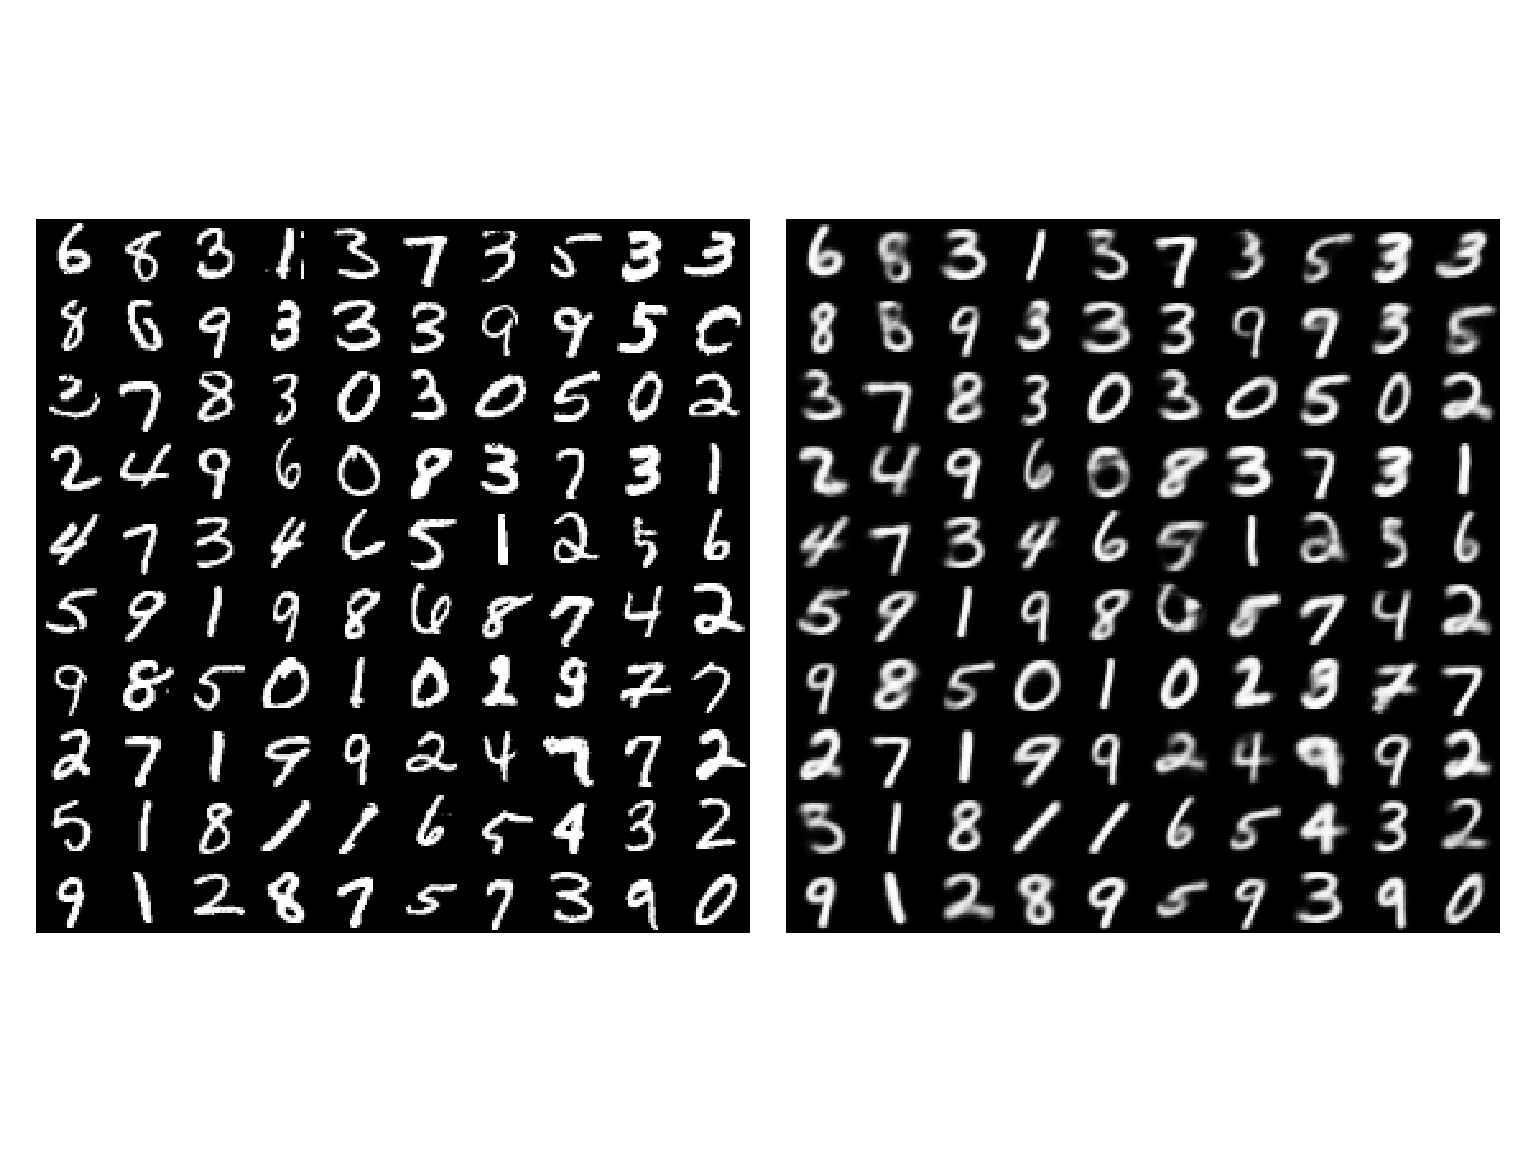
\includegraphics[height=200px, trim={2cm 2cm 2cm 2cm}, clip]{includes/plots/gumbolt-vae/mnist/regenerated.png}
		\caption{Reconstruction Plot for Gumbolt-Vae}
		\label{fig:recon}
	\end{figure}
	\begin{figure}[htpb]
		\centering
		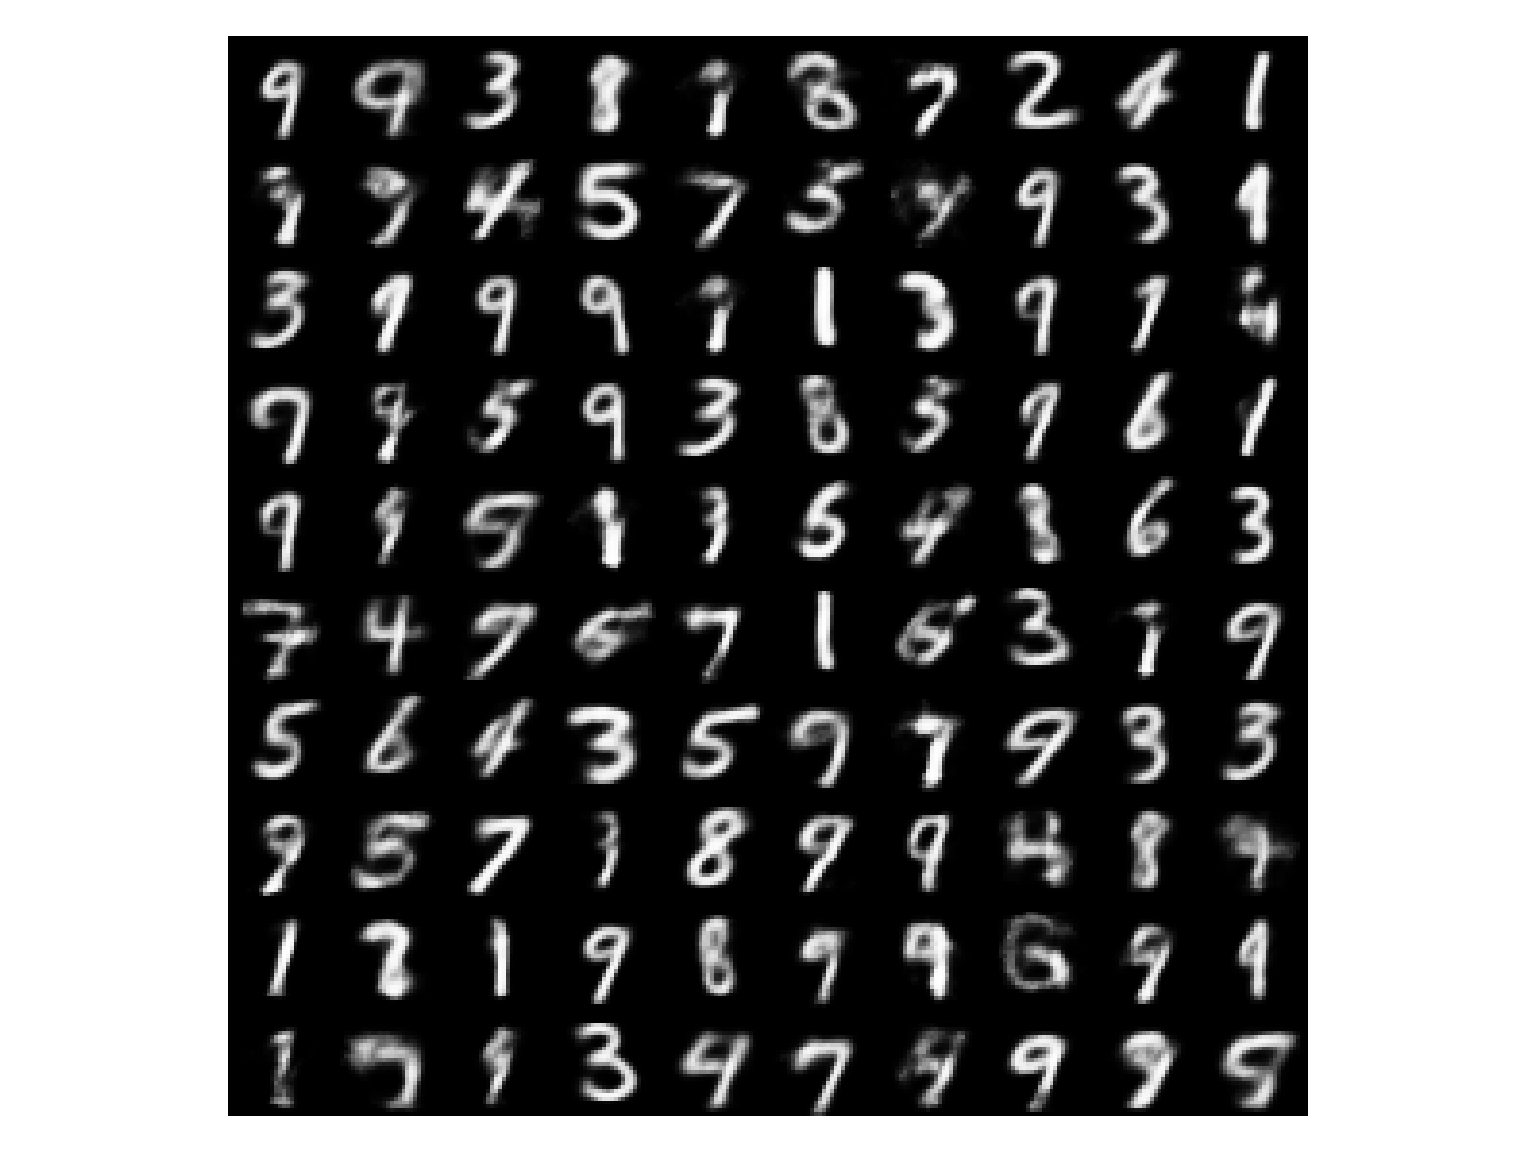
\includegraphics[height=200px]{includes/plots/gumbolt-vae/mnist/sampled.png}
		\caption{Sampling Plot for Gumbolt-Vae}
		\label{fig:sample}
	\end{figure}

	The results of the Gumbolt-VGAE compared to baselines for link prediction on datasets Citeseer and Cora are shown in table \ref{tab:res}
	\fontsize{7.5pt}{7.2}\selectfont
\end{psection}

\newpage

\bibliographystyle{plainnat}
\bibliography{report}

\end{document}
